%%-----------------------------------------------
%
% Include for design chapter of dissertation
%
%%----------------------------------------------



\section{ Target Platform \& High Level Considerations }

\subsection{Use Case Analysis}

Given the project objectives identified above, four primary use cases were
identified for Partridge as shown in Figure \ref{fig:use_cases}. Users can be
identified as researchers and people interested in finding and reading
scientific papers that interested them. This would involve querying the
database for relevant papers, viewing metrics on the papers that have been used
to classify them and also downloading the original paper for reading. A subset
of users were identified as authors who might be interested in adding their own
papers to the Partridge instance.

\begin{figure}[!h]
\centering
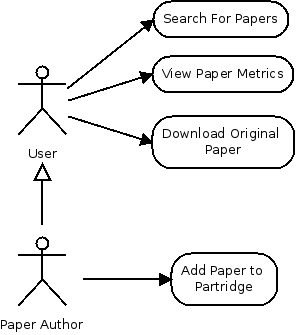
\includegraphics[width=0.4\textwidth]{images/design/use_cases.png}
\caption{Use Case Diagram for Partridge Project}
\label{fig:use_cases}
\end{figure}

\subsection{ Target Platform}

It was decided from the outset that Partridge would be a web-based tool.
Web-based systems can generally be run on any computer with access to the
internet and a modern web browser. This also means that there is no need for
the end user to install or configure extra software on their computers, making
Partridge accessible to non-technical users and those who have aggressive
software restrictions on their computers, such as GPs and users of public
computers in libraries or on academic sites.

In order to function as a website, Partridge needed to be developed as a server
application that produced Hyper Text Markup Language (HTML) output that a web
browser could interpret and display. The browser rendering the forms must then
communicate with a backend system capable of querying and returning papers to
the user based on their input. This lead to the decision to split development
of Partridge into two core components: the Web Frontend comprising of user
interface elements and presentation logic and the Web Backend comprising of
intelligent systems to classify, filter and query papers using some of the NLP
techniques discussed previously.

One of the main requirements for a web server is that it responds to requests
relatively quickly, ideally within 10 seconds or less. If they don't, the user
may get impatient and give up trying to use the system, or in some cases, their
web browser may timeout and stop trying to load the page. Many of the processes
involved in extracting meaningful CoreSC information from papers are very slow
slow. This means that processing papers during web requests is not really
feasible, since it may take several minutes for a single paper to be annotated
and classified. Therefore, a third core component was identified: a paper
preprocessor service that runs on the server and converts, annotates and
classifies papers as soon as they are uploaded.

\subsection{ Programming and Development Environment }

Rather than building a web server from the ground up, most modern web
applications are written in higher level languages that run on top of standard,
open source web servers such as Apache or nginx. Common language choices
include PHP, Python, Perl and Java, all of these languages supported by large
communities of developers and users who provide with excellent documentation
and support if required.  For the implementation of Partridge, Python was
selected as the programming language of choice. This was partially due to the
author's familiarity with the language and also due to the availability of
stable data mining\cite{curk05} and natural language
processing\cite{bird2009natural} libraries for the Python programming
environment. Python is an interpreted cross-platform language, minimising
deployment problems and supports natively compiled C and C++ extension
libraries allowing intensive processing  and number crunching to be offloaded
to native plugins, increasing application processing speed.

To further increase development speed, a Python framework for developing web
applications called \emph{Flask\cite{flask2012}} would be used to build the web
backend.

The development of the application would be carried out on a Linux desktop
computer. However, the portable nature of Python, Apache and the required
libraries meant that Partridge could theoretically be deployed to Windows and
Mac computer systems if required.

The Web Frontend for the system would need to be written using a combination of
HTML markup and JavaScript. HTML is not a programming language in itself and
doesn't contain any logic. It is merely a code representation of the interface
to be rendered in the browser window which is interpreted once it has been
downloaded from the web server. In order to carry out actions on the HTML such
as validating user input and manipulating parts of the display, JavaScript is
also downloaded from the web server and interpreted by the browser. Although
this requires the developer to have knowledge of two extra technologies on top
of Python, it also makes enforcing the design principle of keeping presentation
and logic separate a lot easier.

Due to the large number of popular web browsers on the market, implementing
JavaScript in a slightly different way, Javascript can be very difficult to
write in a cross-browser compatible way.  To maximise compatibility and reduce
development time, it was decided that libraries such as jQuery which are
designed to carry out HTML manipulation behaviours in a uniform way cross all
compatible browsers.  As of February 2013, it is estimated that Chrome and
Firefox are currently the most popular web browsers, holding 50\% and 29.6\% of
the market share respectively\cite{browserstats2013}. Internet Explorer is the
third most popular browser. However, there are several well known compatibility
issues with Internet Explorer, Microsoft themselves condemning version 6.0 of
their browser\cite{ie6death}. For this reason, it was decided that Partridge
would only support Firefox and Chrome. A working interface in modern editions
of the Internet Explorer family of browsers would be a bonus.  However, no time
was allocated to ensuring compatibility of Partridge with Internet Explorer.

\section{ System Architecture }


\begin{figure}[!ht]
\center
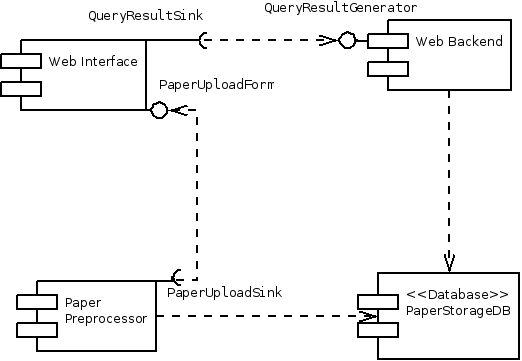
\includegraphics[width=0.9\textwidth]{images/design/components_high_level.png}
\caption{High Level Component Layout for Partridge}
\label{fig:high_level_components}
\end{figure}

Figure \ref{fig:high_level_components} shows a very high level description of
the system's three main components, the database server and the ways that they
communicate. Communication between the Web Interface and the other two
components is carried out via HTTP requests to the underlying Apache server.
Communication between the web backend and the paper preprocessor is implicit
via the data storage system. Direct communication between these components is
redundant since the web backend cannot gain any extra information from the
paper preprocessor while a paper is still being analysed and all finished
papers are added to the database which the web backend has full access to
anyway.

\subsection{ Data Storage }

\subsection{ Preprocessor }

\subsection{ Web Backend }

\subsection{ Web Frontend }
